\documentclass[review]{elsarticle}

\journal{Annals of Nuclear Energy}
%%%% packages and definitions (optional)
\newcommand{\Cyclus}{\textsc{Cyclus}\xspace}%
\newcommand{\Cycamore}{\textsc{Cycamore}\xspace}

\usepackage{lineno}
\usepackage{tabularx}
\usepackage[acronym,toc]{glossaries}
%\newacronym{<++>}{<++>}{<++>}
\newacronym[longplural={metric tons of heavy metal}]{MTHM}{MTHM}{metric ton of heavy metal}
\newacronym{ABM}{ABM}{agent-based modeling}
\newacronym{ACDIS}{ACDIS}{Program in Arms Control \& Domestic and International Security}
\newacronym{AHTR}{AHTR}{Advanced High Temperature Reactor}
\newacronym{ANDRA}{ANDRA}{Agence Nationale pour la gestion des D\'echets RAdioactifs, the French National Agency for Radioactive Waste Management}
\newacronym{ANL}{ANL}{Argonne National Laboratory}
\newacronym{ANS}{ANS}{American Nuclear Society}
\newacronym{API}{API}{application programming interface}
\newacronym{ARE}{ARE}{Aircraft Reactor Experiment}
\newacronym{ARFC}{ARFC}{Advanced Reactors and Fuel Cycles}
\newacronym{ASME}{ASME}{American Society of Mechanical Engineers}
\newacronym{ATWS}{ATWS}{Anticipated Transient Without Scram}
\newacronym{BDBE}{BDBE}{Beyond Design Basis Event}
\newacronym{BIDS}{BIDS}{Berkeley Institute for Data Science}
\newacronym{CAFCA}{CAFCA}{ Code for Advanced Fuel Cycles Assessment }
\newacronym{CDTN}{CDTN}{Centro de Desenvolvimento da Tecnologia Nuclear}
\newacronym{CEA}{CEA}{Commissariat \`a l'\'Energie Atomique et aux \'Energies Alternatives}
\newacronym{CI}{CI}{continuous integration}
\newacronym{CNEN}{CNEN}{Comiss\~{a}o Nacional de Energia Nuclear}
\newacronym{CNERG}{CNERG}{Computational Nuclear Engineering Research Group}
\newacronym{COSI}{COSI}{Commelini-Sicard}
\newacronym{COTS}{COTS}{commercial, off-the-shelf}
\newacronym{CSNF}{CSNF}{commercial spent nuclear fuel}
\newacronym{CTAH}{CTAHs}{Coiled Tube Air Heaters}
\newacronym{CUBIT}{CUBIT}{CUBIT Geometry and Mesh Generation Toolkit}
\newacronym{CURIE}{CURIE}{Centralized Used Fuel Resource for Information Exchange}
\newacronym{DAG}{DAG}{directed acyclic graph}
\newacronym{DANESS}{DANESS}{Dynamic Analysis of Nuclear Energy System Strategies}
\newacronym{DBE}{DBE}{Design Basis Event}
\newacronym{DESAE}{DESAE}{Dynamic Analysis of Nuclear Energy Systems Strategies}
\newacronym{DHS}{DHS}{Department of Homeland Security}
\newacronym{DOE}{DOE}{Department of Energy}
\newacronym{DRACS}{DRACS}{Direct Reactor Auxiliary Cooling System}
\newacronym{DRE}{DRE}{dynamic resource exchange}
\newacronym{DSNF}{DSNF}{DOE spent nuclear fuel}
\newacronym{DYMOND}{DYMOND}{Dynamic Model of Nuclear Development }
\newacronym{EBS}{EBS}{Engineered Barrier System}
\newacronym{EDF}{EDF}{Électricité de France}
\newacronym{EDZ}{EDZ}{Excavation Disturbed Zone}
\newacronym{EIA}{EIA}{U.S. Energy Information Administration}
\newacronym{EPA}{EPA}{Environmental Protection Agency}
\newacronym{EP}{EP}{Engineering Physics}
\newacronym{FCO}{FCO}{Fuel Cycle Options}
\newacronym{FCT}{FCT}{Fuel Cycle Technology}
\newacronym{FEHM}{FEHM}{Finite Element Heat and Mass Transfer}
\newacronym{FEPs}{FEPs}{Features, Events, and Processes}
\newacronym{FHR}{FHR}{Fluoride-Salt-Cooled High-Temperature Reactor}
\newacronym{FLiBe}{FLiBe}{Fluoride-Lithium-Beryllium}
\newacronym{GDSE}{GDSE}{Generic Disposal System Environment}
\newacronym{GDSM}{GDSM}{Generic Disposal System Model}
\newacronym{GENIUSv1}{GENIUSv1}{Global Evaluation of Nuclear Infrastructure Utilization Scenarios, Version 1}
\newacronym{GENIUSv2}{GENIUSv2}{Global Evaluation of Nuclear Infrastructure Utilization Scenarios, Version 2}
\newacronym{GENIUS}{GENIUS}{Global Evaluation of Nuclear Infrastructure Utilization Scenarios}
\newacronym{GPAM}{GPAM}{Generic Performance Assessment Model}
\newacronym{GRSAC}{GRSAC}{Graphite Reactor Severe Accident Code}
\newacronym{GUI}{GUI}{graphical user interface}
\newacronym{HLW}{HLW}{high level waste}
\newacronym{HPC}{HPC}{high-performance computing}
\newacronym{HTC}{HTC}{high-throughput computing}
\newacronym{HTGR}{HTGR}{High Temperature Gas-Cooled Reactor}
\newacronym{IAEA}{IAEA}{International Atomic Energy Agency}
\newacronym{IEMA}{IEMA}{Illinois Emergency Mangament Agency}
\newacronym{IHLRWM}{IHLRWM}{International High Level Radioactive Waste Management}
\newacronym{INL}{INL}{Idaho National Laboratory}
\newacronym{IPRR1}{IRP-R1}{Instituto de Pesquisas Radioativas Reator 1}
\newacronym{IRP}{IRP}{Integrated Research Project}
\newacronym{ISFSI}{ISFSI}{Independent Spent Fuel Storage Installation}
\newacronym{ISRG}{ISRG}{Independent Student Research Group}
\newacronym{JFNK}{JFNK}{Jacobian-Free Newton Krylov}
\newacronym{LANL}{LANL}{Los Alamos National Laboratory}
\newacronym{LBNL}{LBNL}{Lawrence Berkeley National Laboratory}
\newacronym{LCOE}{LCOE}{levelized cost of electricity}
\newacronym{LDRD}{LDRD}{laboratory directed research and development}
\newacronym{LFR}{LFR}{Lead-Cooled Fast Reactor}
\newacronym{LLNL}{LLNL}{Lawrence Livermore National Laboratory}
\newacronym{LMFBR}{LMFBR}{Liquid Metal Fast Breeder Reactor}
\newacronym{LOFC}{LOFC}{Loss of Forced Cooling}
\newacronym{LOHS}{LOHS}{Loss of Heat Sink}
\newacronym{LOLA}{LOLA}{Loss of Large Area}
\newacronym{LP}{LP}{linear program}
\newacronym{LWR}{LWR}{Light Water Reactor}
\newacronym{MA}{MA}{minor actinide}
\newacronym{MAGNOX}{MAGNOX}{Magnesium Alloy Graphie Moderated Gas Cooled Uranium Oxide Reactor}
\newacronym{MCNP}{MCNP}{Monte Carlo N-Particle code}
\newacronym{MILP}{MILP}{mixed-integer linear program}
\newacronym{MIT}{MIT}{the Massachusetts Institute of Technology}
\newacronym{MOAB}{MOAB}{Mesh-Oriented datABase}
\newacronym{MOOSE}{MOOSE}{Multiphysics Object-Oriented Simulation Environment}
\newacronym{MOX}{MOX}{mixed oxide}
\newacronym{MSBR}{MSBR}{Molten Salt Breeder Reactor}
\newacronym{MSRE}{MSRE}{Molten Salt Reactor Experiment}
\newacronym{MSR}{MSR}{Molten Salt Reactor}
\newacronym{NAGRA}{NAGRA}{National Cooperative for the Disposal of Radioactive Waste}
\newacronym{NEAMS}{NEAMS}{Nuclear Engineering Advanced Modeling and Simulation}
\newacronym{NEUP}{NEUP}{Nuclear Energy University Programs}
\newacronym{NFCSim}{NFCSim}{Nuclear Fuel Cycle Simulator}
\newacronym{NGNP}{NGNP}{Next Generation Nuclear Plant}
\newacronym{NMWPC}{NMWPC}{Nuclear MW Per Capita}
\newacronym{NNSA}{NNSA}{National Nuclear Security Administration}
\newacronym{NPRE}{NPRE}{Department of Nuclear, Plasma, and Radiological Engineering}
\newacronym{NQA1}{NQA-1}{Nuclear Quality Assurance - 1}
\newacronym{NRC}{NRC}{Nuclear Regulatory Commission}
\newacronym{NSF}{NSF}{National Science Foundation}
\newacronym{NSSC}{NSSC}{Nuclear Science and Security Consortium}
\newacronym{NUWASTE}{NUWASTE}{Nuclear Waste Assessment System for Technical Evaluation}
\newacronym{NWF}{NWF}{Nuclear Waste Fund}
\newacronym{NWTRB}{NWTRB}{Nuclear Waste Technical Review Board}
\newacronym{OCRWM}{OCRWM}{Office of Civilian Radioactive Waste Management}
\newacronym{ORION}{ORION}{ORION}
\newacronym{ORNL}{ORNL}{Oak Ridge National Laboratory}
\newacronym{PARCS}{PARCS}{Purdue Advanced Reactor Core Simulator}
\newacronym{PBAHTR}{PB-AHTR}{Pebble Bed Advanced High Temperature Reactor}
\newacronym{PBFHR}{PB-FHR}{Pebble-Bed Fluoride-Salt-Cooled High-Temperature Reactor}
\newacronym{PEI}{PEI}{Peak Environmental Impact}
\newacronym{PH}{PRONGHORN}{PRONGHORN}
\newacronym{PRIS}{PRIS}{Power Reactor Information System}
\newacronym{PRKE}{PRKE}{Point Reactor Kinetics Equations}
\newacronym{PSPG}{PSPG}{Pressure-Stabilizing/Petrov-Galerkin}
\newacronym{PWAR}{PWAR}{Pratt and Whitney Aircraft Reactor}
\newacronym{PWR}{PWR}{Pressurized Water Reactor}
\newacronym{PyNE}{PyNE}{Python toolkit for Nuclear Engineering}
\newacronym{PyRK}{PyRK}{Python for Reactor Kinetics}
\newacronym{QA}{QA}{quality assurance}
\newacronym{RDD}{RD\&D}{Research Development and Demonstration}
\newacronym{RD}{R\&D}{Research and Development}
\newacronym{RELAP}{RELAP}{Reactor Excursion and Leak Analysis Program}
\newacronym{RIA}{RIA}{Reactivity Insertion Accident}
\newacronym{RIF}{RIF}{Region-Institution-Facility}
\newacronym{SFR}{SFR}{Sodium-Cooled Fast Reactor}
\newacronym{SINDAG}{SINDA{\textbackslash}G}{Systems Improved Numerical Differencing Analyzer $\backslash$ Gaski}
\newacronym{SKB}{SKB}{Svensk K\"{a}rnbr\"{a}nslehantering AB}
\newacronym{SNF}{SNF}{spent nuclear fuel}
\newacronym{SNL}{SNL}{Sandia National Laboratory}
\newacronym{STC}{STC}{specific temperature change}
\newacronym{SUPG}{SUPG}{Streamline-Upwind/Petrov-Galerkin}
\newacronym{SWF}{SWF}{Separations and Waste Forms}
\newacronym{SWU}{SWU}{Separative Work Unit}
\newacronym{TRIGA}{TRIGA}{Training Research Isotope General Atomic}
\newacronym{TRISO}{TRISO}{Tristructural Isotropic}
\newacronym{TSM}{TSM}{Total System Model}
\newacronym{TSPA}{TSPA}{Total System Performance Assessment for the Yucca Mountain License Application}
\newacronym{ThOX}{ThOX}{thorium oxide}
\newacronym{UFD}{UFD}{Used Fuel Disposition}
\newacronym{UML}{UML}{Unified Modeling Language}
\newacronym{UOX}{UOX}{uranium oxide}
\newacronym{UQ}{UQ}{uncertainty quantification}
\newacronym{US}{US}{United States}
\newacronym{UW}{UW}{University of Wisconsin}
\newacronym{VISION}{VISION}{the Verifiable Fuel Cycle Simulation Model}
\newacronym{VV}{V\&V}{verification and validation}
\newacronym{VVER}{VVER}{Voda-Vodyanoi Energetichesky Reaktor (Russian Pressurized Water Reactor)}
\newacronym{WIPP}{WIPP}{Waste Isolation Pilot Plant}
\newacronym{YMR}{YMR}{Yucca Mountain Repository Site}

\makeglossaries
\usepackage{xspace}

\usepackage{caption}
\newcolumntype{b}{X}
\newcolumntype{s}{>{\hsize=.5\hsize}X}
\newcolumntype{m}{>{\hsize=.75\hsize}X}



\usepackage{tikz}
\usetikzlibrary{shapes.geometric,arrows}
\tikzstyle{process} = [rectangle, rounded corners, minimum width=3cm, minimum height=1cm,text centered, draw=black, fill=blue!30]
\tikzstyle{object} = [ellipse, rounded corners, minimum width=3cm, minimum height=1cm,text centered, draw=black, fill=green!30]
\tikzstyle{arrow} = [thick,->,>=stealth]
\usetikzlibrary{positioning, arrows, decorations, shapes }%


\begin{document}

\begin{frontmatter}
\title{Standardized Verification of the Cyclus Fuel Cycle Simulator}
\author{Jin Whan Bae$^{1}$, Joshua L. Peterson-Droogh$^{2}$, Kathryn D. Huff$^{1}$}
\address{$^{1}$Dept. of Nuclear, Plasma, and Radiological Engineering, University of Illinois at Urbana-Champaign, Urbana, IL \\ $^{2}$Oak Ridge National Laboratory, Oak Ridge, TN }

\begin{abstract}
Many nuclear fuel cycle simulators can analyze transitions from once-through to 
advanced nuclear fuel cycles. Verification studies compare various fuel 
cycle analysis tools to test agreement and identify sources of difference.  A 
recent verification study, B. Feng et al., ``Standardized verification of fuel 
cycle modeling,'' Annals of Nuclear Energy, vol. 94, pp. 300-312, Aug.  2016 
\cite{feng_standardized_2016} established transition scenario test case 
specifications and accordingly evaluated national laboratory nuclear fuel cycle 
simulators, DYMOND, VISION, ORION, and  MARKAL.  This work verifies the 
performance of \Cyclus, the agent-based, open-source fuel cycle simulator, 
using the test case specifications in Feng et. al.  In this work, \Cyclus 
demonstrates agreement with the results from the previous verification study. 
Minor differences reflect intentional, detailed material tracking in the 
\Cycamore reactor module.  These results extend the example results in Feng et. 
al to further enable future verification of additional nuclear fuel cycle 
simulation tools.  
\end{abstract}


\end{frontmatter}

\modulolinenumbers[5]
\linenumbers
	
\section{Abstract}
Numerous nuclear fuel cycle system modeling codes
have been developed to perform fuel cycle transition
analyses from a once-through cycle to an advanced
fuel cycle. Verification studies compare different
fuel cycle analysis tools against each other to
test agreement and identify sources of difference.
This paper benchmarks \Cyclus, the agent-based,
open-source fuel cycle simulation code, against
a verification study \cite{feng_standardized_2016} with
DYMOND \cite{yacout_modeling_2005},
VISION \cite{jacobson_verifiable_2010},
ORION \cite{gregg_analysis_2012}, and
MARKAL \cite{shay_epa_2006}. The study reveals
that \Cyclus' results match the spreadsheet results
very closely, with minor differences caused by
reactor module behavior.

\section{Introduction}
Fuel cycle simulators act as an important tool to
aid decision in policy and fuel cycle strategies.
To meet this need from various institutions, a
multitude of fuel cycle simulators were developed,
using different methods and different structures
to simulate the material flow in the nuclear fuel cycle.
The difference in the algorithm of fuel cycle analysis
codes combined with a small user community make
validation studies necessary to gain
confidence of the capability of the code as well as its
agreement with other analysis codes.

This study is done to benchmark \Cyclus' results
against that of other well-known codes, such as
DYMOND \cite{yacout_modeling_2005},
VISION \cite{jacobson_verifiable_2010},
ORION \cite{gregg_analysis_2012}, and
MARKAL \cite{shay_epa_2006}. We take the input
parameters and results from a validation study
\cite{feng_standardized_2016} already done for the
mentioned tools for a transition scenario from an
open fuel cycle to an advanced fuel cycle with
reprocessing. In the paper, the `model solutions'
generated from an excel worksheet are compared
with each code results, and the results show
excellent agreement.


\subsection{\Cyclus}

\Cyclus is an agent-based fuel cycle simulation framework 
\cite{huff_fundamental_2016}, which means 
that each reactor, reprocessing plant, and fuel fabrication plant is modeled as an agent.
A \Cyclus simulation contains prototypes, which are fuel cycle facilities with
pre-defined parameters, that are deployed in the simulation as \texttt{facility} agents.
Encapsulating the \texttt{facility} agents are the \texttt{Institution} and \texttt{Region}.
A \texttt{Region} agent holds a set of \texttt{Institution}s.
An \texttt{Institution} agent can deploy or decommission \texttt{facility} agents.
The \texttt{Institution} agent is part of a \texttt{Region} agent,
which can contain multiple \texttt{Institution} agents. Several versions of \texttt{Institution}
and \texttt{Region} exist, varying in complexity and functions \cite{huff_extensions_2014}.
 \texttt{DeployInst} is used as the institution archetype for this work, where the institution
deploys agents at user-defined timesteps.

At each timestep (one month),
agents make requests for materials or bid to supply them and exchange
with one another. A market-like mechanism called the dynamic resource exchange
\cite{gidden_agent-based_2015} governs the exchanges.
Each material resource has a quantity, composition, name, and a unique identifier
for output analysis. The timestep execution in \Cyclus follows 
\texttt{Build, Tick, \gls{DRE}, Tock, and Decommission}, as illustrated in
figure \ref{fig:time}. The \texttt{Tick}, and \texttt{Tock} phases are for
each agent to perform actions, such as transmutation, separation, generation,
of materials before and after the market exchange phase. 

\begin{figure}[h]
\centering
\scalebox{0.7}{
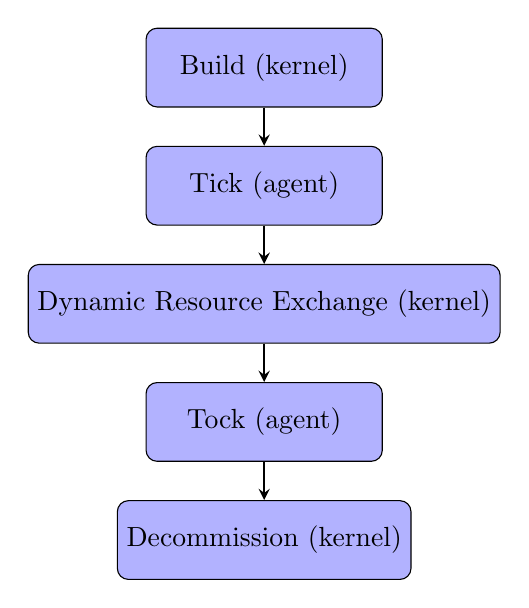
\begin{tikzpicture}[node distance=1.5cm]
\node (Build) [process] {Build (kernel)};
\node (Tick) [process, below of=Build] {Tick (agent)};
\node (DRE) [process, below of=Tick]{Dynamic Resource Exchange (kernel) };
\node (Tock) [process, below of=DRE]{Tock (agent)};
\node (Decom) [process, below of=Tock] {Decommission (kernel)};

\draw [arrow] (Build) -- (Tick); 
\draw [arrow] (Tick) -- (DRE);
\draw [arrow] (DRE) -- (Tock);
\draw [arrow] (Tock) -- (Decom);
\end{tikzpicture}
}
\caption{\Cyclus timestep execution steps.}
\label{fig:time}
\end{figure}

The modularity of \Cyclus allows a low barrier of
entry for developers, since developers can create an
archetype (e.g. Reactor module, Reprocessing module)
without extensive knowledge of the \Cyclus framework.

\section{Methodology}

Feng et al. comprehensively defines simulation parameters
sufficient to reproduce the transition scenario in \Cyclus.
In this study, we used the \Cycamore \cite{huff_fundamental_2016}
 archetype library to model
all fuel cycle facilities. \Cycamore libraries contain
simple fuel cycle facility models. 

\Cyclus results are output in either \texttt{.sqlite} or
\texttt{.h5} format. In this study, we used the
\texttt{.sqlite} format and analyzed the results
using a python script. The post-processed
output data, was overlapped with the results with the
model solution from the verification study \cite{feng_standardized_2016}.
The input file and analysis procedures are all available on Github \cite{bae_arfc/transition-scenarios:_2018}.

The analysis and benchmark were performed iteratively,
where we improve the original result by communicating
with the authors of the benchmark. 
We analyzed the reasons for the differences from the original
result, and made small edits in the source code.
Major differences in the facility behavior algorithms were not edited but
simply explained in detail as to how they contributed
to the difference in the results.


\section{Fundamental Code Differences in \Cyclus}

\Cyclus has fundamental code differences than some fuel cycle analysis codes
used in the benchmark \cite{feng_standardized_2016}.

\Cyclus has a default timestep of a month. In order to take
this into account, we calculate the annual value
(i.e. average value for inventory values and sum of 12 months
for throughput values) for each result. The timestep in \Cyclus
can be changed into a year without changing the source
code, but \Cyclus' timestep execution (figure \ref{fig:time}) causes a delay
in the material flow. Thus, having the timestep be 12 months
allows the lessening of the impact of the delay due to the
\Cyclus timestep execution.

Similarly, \Cyclus has discrete
execution steps per timestep that might cause delays or contort
the results from other simulators. For example, decommissioning of
facilities occur at the end of a timestep, while building of facilities
occur at the beginning of a timestep.

The \Cycamore recipe reactor depletes half of its core when decommissioned,
whereas the codes in the benchmark \cite{feng_standardized_2016} deplete all its fuel when decommissioned. This causes a major
discrepancy for \gls{TRU} inventory. For this study, we changed
the \Cycamore source code to deplete all its assemblies to the depleted recipe.
Also, the \Cycamore recipe reactor treats each batch (and assembly) as a discrete
material, while some codes have continuous fuel discharge. This produces
differences in the results because the batches in the benchmark \cite{feng_standardized_2016} are in fractions.
In this study, the \gls{LWR} batch size and cycle time is increased, while
decreasing the batch number to keep the core size constant. We simply round
up the \gls{SFR} batch number, while the batch size and cycle time are kept constant.
This increases the core size by $1.08 \%$, which is negligible, but will be
discussed in the results section.
We list the differences in table \ref{tab:diff}.

\begin{table}[h]
    \centering
    \caption{Difference in Batch number and core size}
\begin{tabularx}{0.47\textwidth}{bss}
        \hline
        \textbf{Category} & \textbf{Benchmark \cite{feng_standardized_2016}} & \textbf{This study} \\
        \hline
        LWR Batches & 4.5 & 3 \\
        LWR Batch size [tHM] & 19.91 & 29.86 \\
        LWR Core size [tHM] & 89.59 & 89.59 \\
        LWR Cycle time & 1 year & 1.5 years \\
        SFR Batches & 3.96 & 4 \\
        SFR Batch size [tHM] & 3.95 & 3.95 \\
        SFR Core size [tHM] & 15.63 & 15.8 \\
        \hline
        \end{tabularx}
        \label{tab:diff}
\end {table}

Note that all the differences could have been mediated by changing the
archetype source codes. However, the only change made was the reactor
depletion behavior at decommission due to its large impact. Note that the
goal of this
study is to show current \Cyclus agreement with other codes and identify
differences, not to alter \Cyclus to match the other codes.
\section{Results}

Each \Cyclus result is shown as a solid line, and the excel solution in the
paper is shown as a dotted line, for better visualization. The results are
simply a reproduction of the plots displayed in the paper. The excel
results are obtained by personal contact with the paper author
Bo Feng at Argonne National Laboratory.

Most results from \Cyclus show excellent agreement. Differences in results
stem from the errors associated with averaging and the concept of what
constitutes a `snapshot' of a facility inventory.

The deployed reactor capacity is shown in figure \ref{fig:pow_plot}.
The \gls{LWR} retirement and \gls{SFR} deployment timeseries are shown
in figure \ref{fig:dep}. The two plots show exact agreement with the
excel solutions from the paper.

\begin{figure}[htbp!]
	\begin{center}
		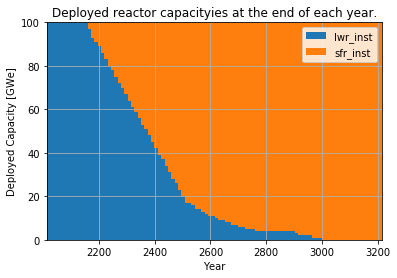
\includegraphics[scale=0.6]{./images/results_18/power_plot.png}
	\end{center}
        \caption{Deployed reactor capacities at the end of each year.}
	\label{fig:pow_plot}
\end{figure}



\begin{figure}[htbp!]
	\begin{center}
		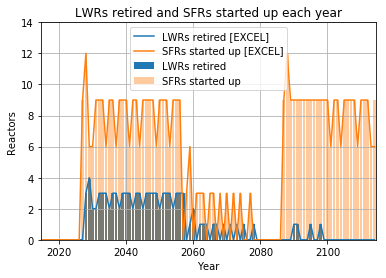
\includegraphics[scale=0.6]{./images/results_18/dep.png}
	\end{center}
        \caption{\glspl{LWR} retired and \glspl{SFR} started up each year.}
	\label{fig:dep}
\end{figure}


The annual fuel loading rates are shown in table \ref{fig:fuel_load}.
The initial fuel loading for 100 \gls{LWR} reactors were edited to match
the plot in the verification
study results. Note the oscillations for the \gls{LWR} fuel loading
is caused by the refueling period being 18-month refuel cycle for all \gls{LWR} reactors
aggregated into 12-month groups. Note also that the total values
are equal for both plots.

Although indistinguishable,
there is a small difference with \gls{SFR} fuel loading, that is proportional
to the core mass difference, as mentioned in the previous section.
Figure \ref{fig:fuel_load_diff_norm} shows the
differences normalized by the core mass differences, overlapped with the
\gls{SFR} deployment. This is to show that the differences only occur during
deployment due to the difference in core mass.


\begin{figure}[htbp!]
    \begin{center}
        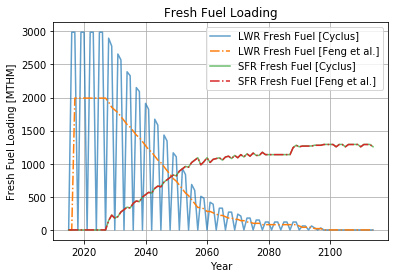
\includegraphics[scale=0.6]{./images/results_18/fuel_load.png}
    \end{center}
        \caption{Annual fresh fuel loading rates (first cores and reload fuel).}
    \label{fig:fuel_load}
\end{figure}


\begin{figure}[htbp!]
    \begin{center}
        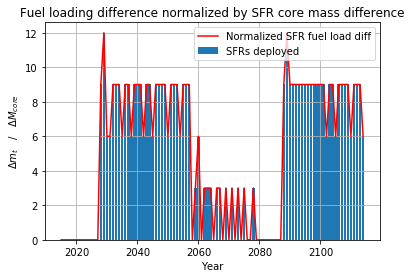
\includegraphics[scale=0.6]{./images/results_18/fuel_load_diff_norm.png}
    \end{center}
        \caption{Difference of annual fresh fuel loading rates (Cyclus - Excel) normalized by the core mass difference of an \gls{SFR} due to fractional batch size.}
    \label{fig:fuel_load_diff_norm}
\end{figure}


The inventory of discharged \gls{UNF} in mandatory cooling stage is shown
in figure \ref{fig:fuel_discharge}. It also oscillates between the excel solution,
and converges. This is due to the annual averaging of
the \gls{UNF} inventory. For a better visual, the monthly inventory is shown
in figure \ref{fig:fuel_discharge_monthly}, where the oscillation is more obvious.
Note that for most plots the \gls{SFR} inventory and fuel loading is almost
exactly the same as the excel solutions, minus the small difference due to core
size.

\begin{figure}[htbp!]
    \begin{center}
        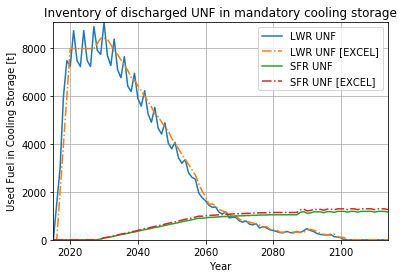
\includegraphics[scale=0.6]{./images/results_18/fuel_discharge.png}
    \end{center}
        \caption{Inventory of discharged \gls{UNF} in mandatory cooling storage.}
    \label{fig:fuel_discharge}
\end{figure}


\begin{figure}[htbp!]
    \begin{center}
        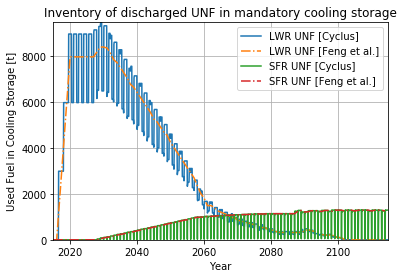
\includegraphics[scale=0.6]{./images/results_18/fuel_discharge_monthly.png}
    \end{center}
        \caption{Inventory of discharged \gls{UNF} in mandatory cooling storage.}
    \label{fig:fuel_discharge_monthly}
\end{figure}


Similar results are shown in figure \ref{fig:waiting} for the inventory of discharge fuel cooled and waiting
for reprocessing. Non-aggregated monthly values are shown in figure \ref{fig:waiting_monthly}.
However, note that the oscillation peaks meet with the excel
solution.  This is because cooled inventory is measured by the cumulative sum
of fuel that has been cooled minus the fuel reprocessed at that timestep.
The cooled inventory before the fuel are sent to reprocessing, which correspond
to the peaks in the oscillation, are the cooled inventory defined by the paper.

\begin{figure}[htbp!]
    \begin{center}
        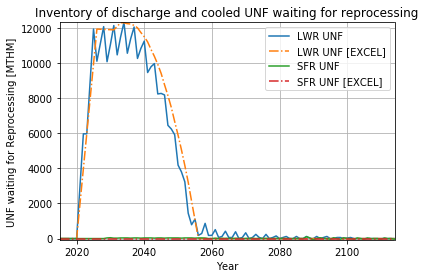
\includegraphics[scale=0.6]{./images/results_18/waiting.png}
    \end{center}
        \caption{Inventory of discharged and cooled \gls{UNF} waiting for reprocessing}
    \label{fig:waiting}
\end{figure}

\begin{figure}[htbp!]
    \begin{center}
        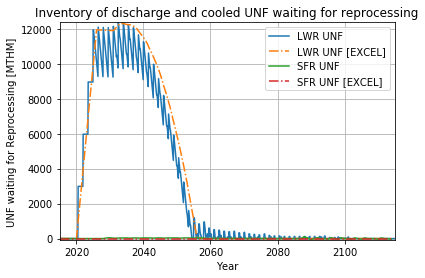
\includegraphics[scale=0.6]{./images/results_18/waiting_monthly.png}
    \end{center}
        \caption{Inventory of discharged and cooled \gls{UNF} waiting for reprocessing.}
    \label{fig:waiting_monthly}
\end{figure}


Figure \ref{fig:rep} shows the reprocessing throughput, which also oscillates between
the excel solution. Note that there is no oscillation in the beginning because the
\gls{LWR} reprocessing plant throughput is maximized at 2,000 tons per year. 

\begin{figure}[htbp!]
    \begin{center}
        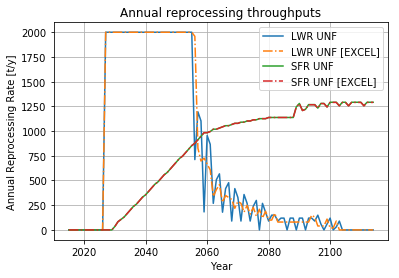
\includegraphics[scale=0.6]{./images/results_18/rep.png}
    \end{center}
        \caption{Annual reprocessing throughputs.}
    \label{fig:rep}
\end{figure}


Figure \ref{fig:tru} shows the inventory of unused \gls{TRU} recovered from \gls{UNF}.
The \Cyclus results follows the excel solutions closely. However, the difference
in core size causes \Cyclus results to be smaller, since more \gls{TRU} is used to
start up the newly deployed \glspl{SFR}. As the \glspl{SFR} \gls{UNF} is used to
create \gls{SFR} fuel, the difference is lessened.

\begin{figure}[htbp!]
	\begin{center}
		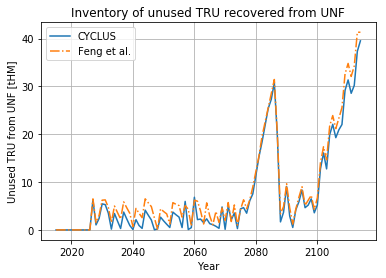
\includegraphics[scale=0.6]{./images/results_18/tru.png}
	\end{center}
        \caption{Inventory of unused \gls{TRU} recovered from \gls{UNF}.}
	\label{fig:tru}
\end{figure}


\section{Discussion}

We benchmarked \Cyclus with results from an established
verification study and saw good agreement
in a transition scenario.

Throughout this work, two major differences were identified
that led to the deviation
of \Cyclus results from that of the benchmark solution. First,
the \Cycamore reactor depletes only half of its core
when decommissioned. Second, \Cyclus, unlike other
codes examined in the benchmark (except ORION), fully resolves
discrete batches for fuel discharge.
We resolve the first discrepancy by changing one line in the source code.

This study proves \Cyclus as a capable tool for modeling
fuel cycle transition scenarios, and shows promise for
expansion and future development.
\section{Acknowledgments}
This work was supported by the Nuclear Engineering Science Laboratory Synthesis 
(NESLS) program as well as the DOE Office of Nuclear Energy's Nuclear Energy 
University Program (Project 16-10512) 'Demand-Driven Cycamore Archetypes'. We 
thank Eva Davidson from Oak Ridge National Laboratory (ORNL) and Bo Feng from 
Argonne National Laboratory (ANL) for their aid in providing benchmark 
solutions and insight for this work. Additionally, the authors are thankful for 
the thoughtful reviews from our colleagues in the Advanced Reactors and Fuel 
Cycles research group.

Prof. Huff is supported by the Nuclear Regulatory Commission Faculty 
Development Program, the Blue Waters sustained-petascale computing project 
supported by the National Science Foundation (awards OCI-0725070 and 
ACI-1238993) and the state of Illinois, the NNSA Office of Defense Nuclear 
Nonproliferation R\&D through the Consortium for Verfication Technologies and 
the Consortium for Nonproliferation Enabling Capabilities (awards DE-NA0002576 
and DE-NA0002534), and the International Institute for Carbon Neutral Energy 
Research (WPI-I2CNER), sponsored by the Japanese Ministry of Education, 
Culture, Sports, Science and Technology.




\bibliographystyle{elsarticle-num}
\bibliography{bibliography}


\end{document}
